\documentclass[conference]{IEEEtran}
\usepackage[utf8]{inputenc}
\usepackage{amsmath,amssymb}
\usepackage{graphicx}
\usepackage{hyperref}
\usepackage{cite}
\usepackage{booktabs}
\usepackage{url}
\usepackage{xcolor}
\usepackage{colortbl}

\renewcommand{\arraystretch}{1.15}

\title{Agentic Search Efficiency for Scientific Data Discovery:\\
A Three-Path Comparison}

\author{
\IEEEauthorblockN{Shazzadul Islam, Jaime Cernuda, Xian-He Sun, Anthony Kougkas}
\IEEEauthorblockA{Illinois Institute of Technology, Chicago, IL, USA\\
\texttt{sislam6@hawk.illinoistech.edu, \{jcernudagarcia, sun, akougkas\}@illinoistech.edu}}
}

\begin{document}
\maketitle

\begin{abstract}
Scientific data search demands reasoning that does not scale: inspecting
what each dataset contains, converting between unit conventions, refining
queries when initial results fall short. AI agents can automate this,
but the cost of running them is rarely examined. A single query can consume nearly a million tokens before producing
an answer.

We present CLIO Search, which implements an observe-decide-act-evaluate
cycle for scientific data. Science-aware operators execute deterministic
SI conversion and formula normalization alongside BM25 and dense search.
CLIO inspects what metadata each corpus provides and adapts accordingly.
Federated search spans heterogeneous HPC backends with agentic
refinement.

We compare three agentic paths over 10~discovery queries against the
National Data Platform (NDP, 341~datasets from NOAA, NASA, ECMWF, and
others) using \texttt{claude-sonnet-4-20250514}. Path~1 uses a Claude
native agent with web search and sub-agent spawning. Path~2 uses
NDP-MCP, exposing catalog search via Model Context Protocol. Path~3 uses
an agent backed by CLIO Search. All three answer 10/10 queries correctly
but cost differs dramatically: the native agent consumes 989K tokens in
50.8~minutes; NDP-MCP consumes
989K tokens in 17.4~minutes; CLIO consumes 474K tokens ($-$52\%) in
4.4~minutes ($-$91\%).

The reduction reflects two factors: smaller context ($\sim$2K tokens per
query versus 989K) and fewer reasoning steps (9/10 queries resolve in a
single invocation). Moving corpus profiling, unit conversion, and
ranking out of the LLM's reasoning loop into a deterministic layer
preserves accuracy while halving cost. Agentic search benefits from
co-designing specialized retrieval with the agent over raw catalog
access.
\end{abstract}

\section{Introduction}

Scientific data catalogs are growing faster than human scientists can
browse them. The National Data Platform (NDP)~\cite{ndp2024} federates
hundreds of repositories; IOWarp and other HPC storage platforms expose
billions of objects. AI agents are an increasingly popular way to search
these catalogs: the agent reads the query, calls tools, reads results,
and produces a ranked list of candidate datasets. This workflow is
attractive because it hides the complexity of heterogeneous catalogs
behind a single natural-language interface.

However, the cost of running these agents is rarely measured. Each tool
call injects results into the LLM's context window; each sub-agent spawn
doubles or triples token consumption. When the catalog is large or the
query requires iteration, a single query can consume hundreds of
thousands of tokens and minutes of wall time. Scaling agentic data
discovery to facility-wide catalogs requires understanding where this
cost comes from and how to reduce it.

We present CLIO Search~\cite{clio2026}, which implements an
observe-decide-act-evaluate cycle for scientific data. Science-aware
operators execute deterministic SI conversion and formula normalization
alongside BM25 and dense search. CLIO inspects what metadata each corpus
provides and adapts accordingly. Federated search spans heterogeneous
HPC backends with agentic refinement. In this work, we evaluate one
dimension of CLIO's design: its effect on agentic search efficiency over
the NDP catalog.

\section{Method}

\textbf{Fixed LLM.} All three paths use
\texttt{claude-sonnet-4-20250514} via the Claude Agent SDK, with the
same system prompt and the same 10 scientific discovery queries covering
temperature, pressure, wind, radiation, and other physical measurements.

\textbf{Path 1: Claude Native Agent.} The agent has access to web
search, file read/write, and sub-agent spawning, but no domain-specific
tools. It must locate NDP datasets by searching the web, reading pages,
and synthesizing findings across sub-agents.

\textbf{Path 2: NDP-MCP.} The agent has access to NDP catalog search
via a Model Context Protocol (MCP)~\cite{mcp2024} server. Each call
returns raw dataset JSON, which the agent parses and re-ranks in context.

\textbf{Path 3: CLIO-backed agent.} The agent queries CLIO Search,
which has indexed the 341 NDP datasets with science-aware metadata
extraction: SI unit canonicalization, measurement ranges, and corpus
profiling. CLIO returns ranked citations rather than raw JSON.

We measure total token consumption (including sub-agent tokens), wall
time, number of tool calls per query, and correctness (whether the agent
returns the expected dataset).

\section{Results}

\begin{table}[!t]
\centering
\caption{Agentic efficiency on 10 NDP discovery queries.
$\Delta$~is relative to the Claude Native Agent.}
\label{tab:results}
\footnotesize
\setlength{\tabcolsep}{4pt}
\renewcommand{\arraystretch}{1.2}
\begin{tabular}{@{}l r r r c@{}}
\toprule
\textbf{Method} & \textbf{Tokens} & \textbf{Tok.\ $\Delta$} & \textbf{Time $\Delta$} & \textbf{Ans.} \\
\midrule
Claude Native Agent & 989{,}417 & ---       & ---       & 10/10 \\
\rowcolor{gray!5}
NDP-MCP             & 988{,}954 & $-$0.05\% & $-$65.68\% & 10/10 \\
\rowcolor{gray!15}
\textbf{CLIO}       & \textbf{474{,}101} & \textbf{$-$52.08\%} & \textbf{$-$91.27\%} & \textbf{10/10} \\
\bottomrule
\end{tabular}
\end{table}

\begin{figure}[!t]
\centering
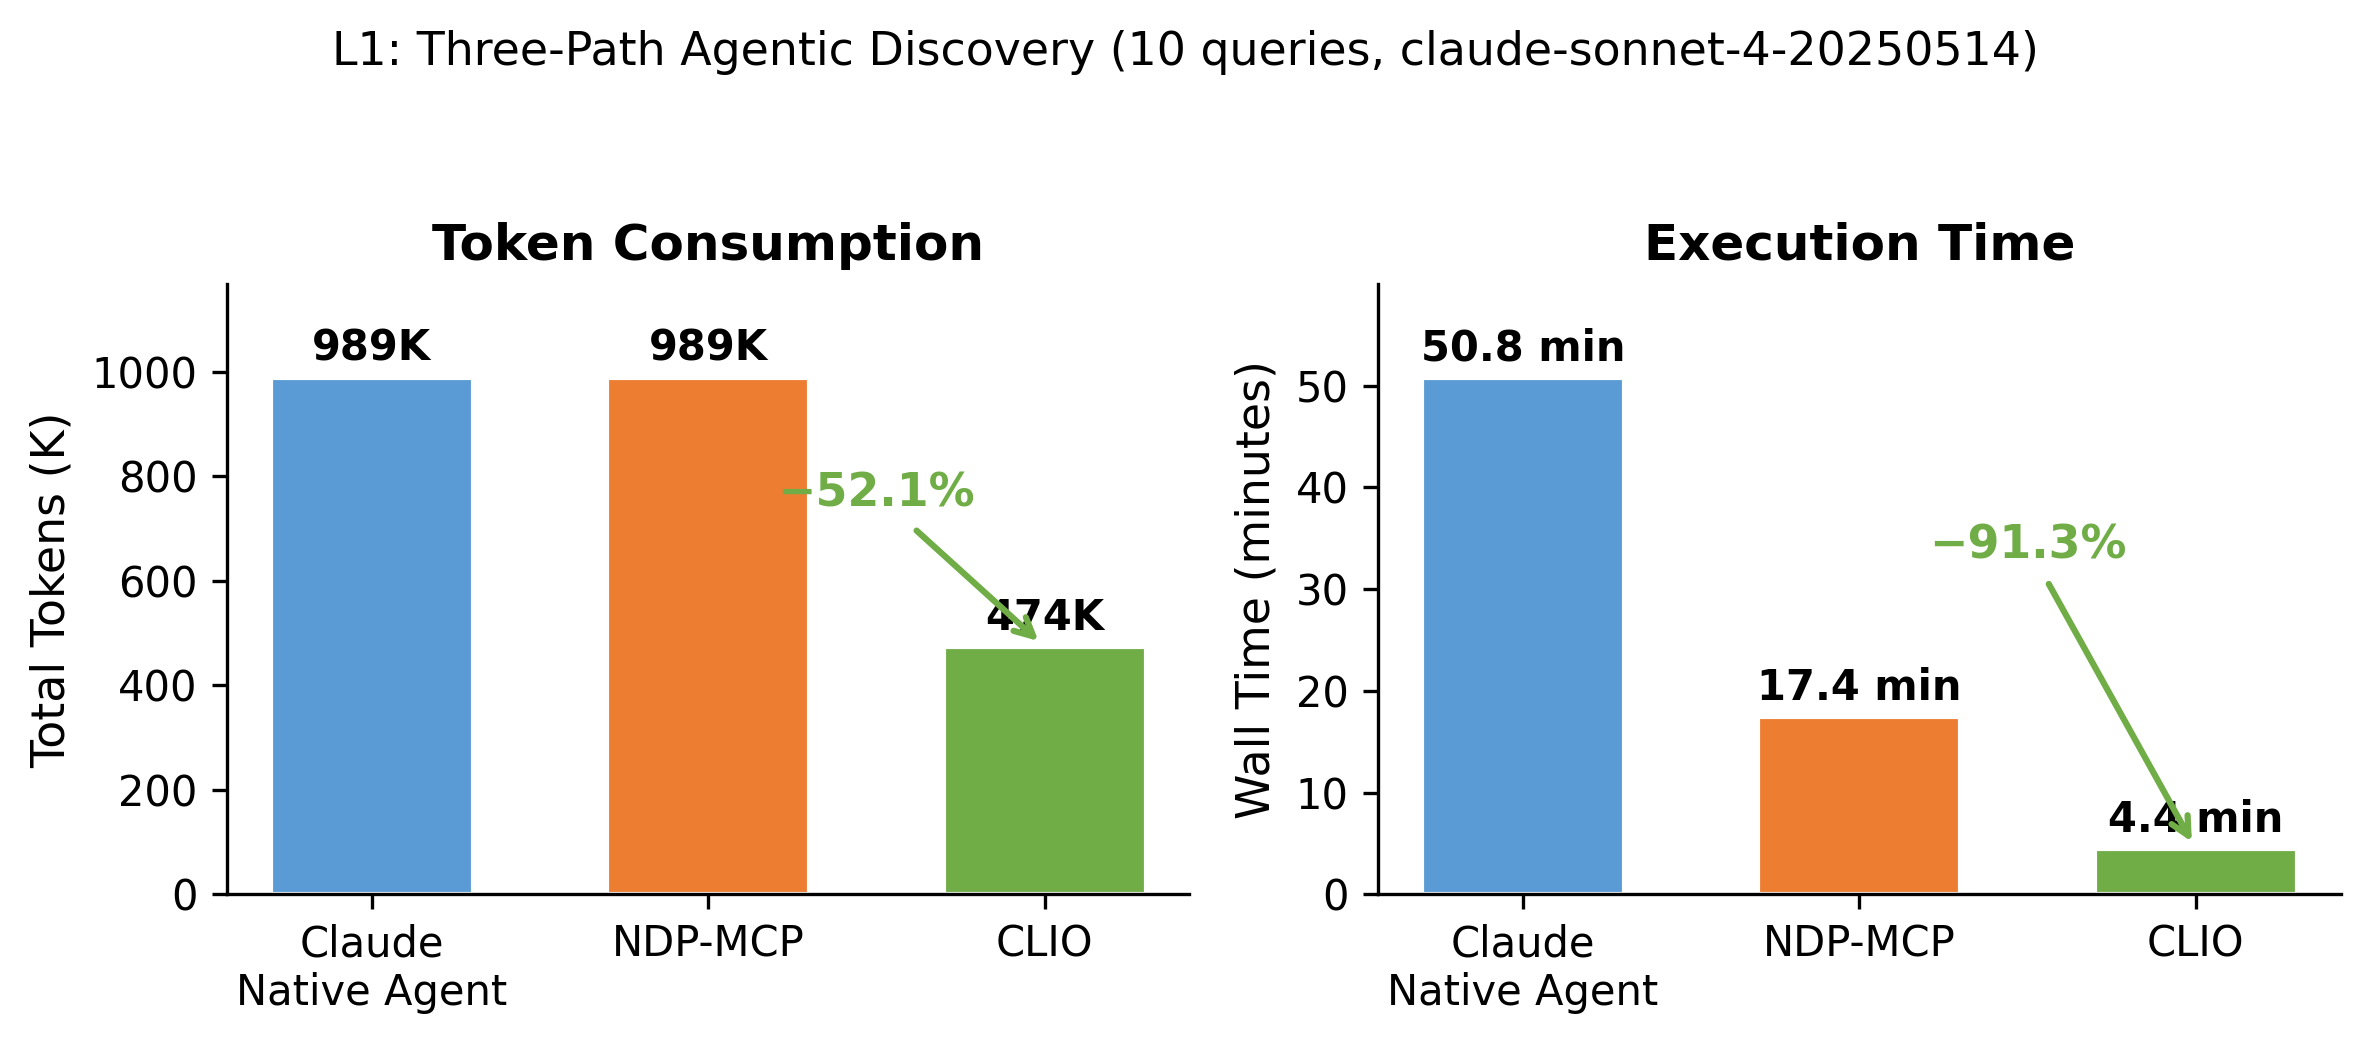
\includegraphics[width=0.95\columnwidth]{fig_L1_three_path.png}
\caption{Token consumption (left) and wall time (right) across 10
queries.}
\label{fig:three-path}
\end{figure}

Table~\ref{tab:results} and Figure~\ref{fig:three-path} report the
results. All three paths answer 10/10 queries correctly, but their
resource consumption differs dramatically. The native agent consumes
989K tokens in 50.8~minutes, averaging 25.6~tool calls per query and
spawning 9~sub-agents (563K main + 426K sub-agent tokens). NDP-MCP
consumes 989K tokens in 17.4~minutes with 7.6~calls per query. CLIO
consumes 474K tokens ($-$52\%) in 4.4~minutes ($-$91\%) with 2~calls per
query, returning $\sim$2K tokens of ranked citations per invocation.

Two factors explain the CLIO reduction. First, \emph{context size}: CLIO
returns structured ranked citations rather than raw catalog JSON,
avoiding hundreds of kilobytes of documents in the agent's context.
Second, \emph{reasoning steps}: 9 of 10 queries resolve in a single
invocation. Only one multi-constraint query required four invocations as
the agent iteratively refined its search terms.

\section{Discussion}

The experiment demonstrates a specific architectural trade-off. Moving
corpus profiling, unit conversion, branch selection, and result ranking
out of the LLM's reasoning loop and into a deterministic local layer
produces substantial savings in both token cost and wall time without
sacrificing accuracy. The effect is larger than exposing the same catalog
through an MCP tool (NDP-MCP), because the MCP tool still injects raw
results that the agent must reason over.

The bottleneck in agentic cost is not the number of tool calls but the
\emph{shape} of the data the agent sees. Compact, ranked, citation-style
results scale better than raw dumps of catalog JSON. Agentic scientific
search benefits from co-designing specialized retrieval with the agent
rather than treating the catalog as an opaque tool.

\begin{thebibliography}{1}
\bibitem{ndp2024}
San Diego Supercomputer Center and University of Utah, ``National Data
Platform: A federated data ecosystem for scientific research,'' 2024, NSF
Award 2333609. [Online]. Available:
\url{https://nationaldataplatform.org}

\bibitem{mcp2024}
Anthropic, ``Introducing the model context protocol,'' 2024. [Online].
Available:
\url{https://www.anthropic.com/news/model-context-protocol}

\bibitem{clio2026}
Authors, ``CLIO Search: Agentic search for scientific data,'' 2026, under
review.
\end{thebibliography}

\end{document}
